\documentclass[colorlinks]{beamer}

\usepackage{babel}
\usepackage{inputenc}
\usepackage{fontenc}

\usepackage{amsmath,amsfonts}

\usepackage{xcolor}
\usepackage{minted}

\newcommand{\norm}[1]{\left\lVert#1\right\rVert}
\newcommand{\myvec}[1]{\ensuremath{\mathbf{#1}}}

\title{IN104: N-Body Problem}
\author{Ismail Bennani\\ismail.lahkim.bennani@ens.fr}

\setbeamertemplate{footline}
{
  \hbox{\begin{beamercolorbox}[wd=1\paperwidth,ht=2.25ex,dp=1ex,right]{framenumber}%
      \usebeamerfont{framenumber}\insertframenumber{} / \inserttotalframenumber\hspace*{2ex}
    \end{beamercolorbox}}%
  \vskip0pt%
}

\begin{document}

\maketitle

\begin{frame}{N-Body Problem}
    Given $N$ bodies at positions $p_i = (x^i, y^i)$ with velocities $v_i = (v_x^i, v_y^i)$, accelerations $a_i = (a_x^i, a_y^i)$ and masses $m_i$, simulate their dynamics and show them on screen. 

    \vspace{1em}

    {\centering DEMO \par}

    \vspace{1em}

    Dynamics of the system:
    \begin{columns}
        \begin{column}{.55\textwidth}
            \begin{equation*}
                \forall i \in [1,N], \left\{\begin{aligned}
                    \ \myvec{\dot{p_i}}(t) & = \myvec{v_i}(t) \\
                    \ \myvec{\dot{v_i}}(t) & = \myvec{a_i}(t) \\
                    \ \myvec{a_i}(t) & = \frac{1}{m_i} \sum_{j \in [1,N], j \ne i} \myvec{F_{i,j}}(t) \\
                \end{aligned}\right.
            \end{equation*}
        \end{column}\hfill\vrule\hfill
        \begin{column}{.4\textwidth}
            where 
            \begin{equation*}
                \myvec{F_{i,j}}(t) = G \frac{m_im_j}{r^2_{i,j}(t)} \myvec{u_{i,j}}(t)
            \end{equation*}
        \end{column}
    \end{columns}
\end{frame}

\begin{frame}{A first implementation}
    \centering DEMO
\end{frame}

\begin{frame}\centering\huge Problem 1: Data structures\end{frame}

\begin{frame}[fragile]{Problem 1: Data structures}
    \footnotesize
    
    
    \begin{columns}
        \begin{column}{.6\textwidth}
        \begin{minted}{python}
bodiesX = [400, 450]
bodiesY = [300, 350]
bodiesVX = [0, 0]
bodiesVY = [0, -0.02]
bodiesMass = [10, 1]
        \end{minted}
        \end{column}
        \begin{column}{.4\textwidth}
            Need a structure to pack the positions, velocities and mass of the body
            
            \centering\textbf{Body}
        \end{column}
    \end{columns}

        \vspace{1em}
        \rule{\textwidth}{0.1pt}

    \begin{columns}
        \begin{column}{.6\textwidth}
        \begin{minted}{python}
diffX = bodiesX[j] - bodiesX[i]
diffY = bodiesY[j] - bodiesY[i]
...
unitX = diffX / norm
unitY = diffY / norm
...
bodiesAX[i] += unitX * G * bodiesMass[i] \
    * bodiesMass[j] / (norm * norm)
bodiesAY[i] += unitY * G * bodiesMass[i] \
    * bodiesMass[j] / (norm * norm)
        \end{minted}
        \end{column}
        \begin{column}{.4\textwidth}
            Need a structure to represent a vector of dim 2 and overriden operators

            \centering\textbf{Vector2}
        \end{column}
    \end{columns}
\end{frame}

\begin{frame}{Data structures}{Body}
    {
        \centering
        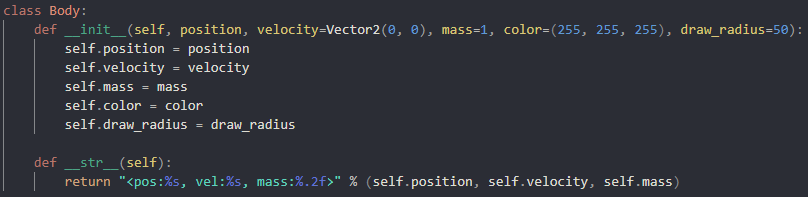
\includegraphics[width=\textwidth]{Body.png}
        \par
    }

    This class is used to pack the data of a body. \\
    
    \mintinline{python}{color} and \mintinline{python}{draw_radius} are used by \mintinline{python}{Screen} to draw the planets.
\end{frame}

\begin{frame}{Data structures}{World}
    \begin{columns}
        \begin{column}{.5\textwidth}
            \centering
            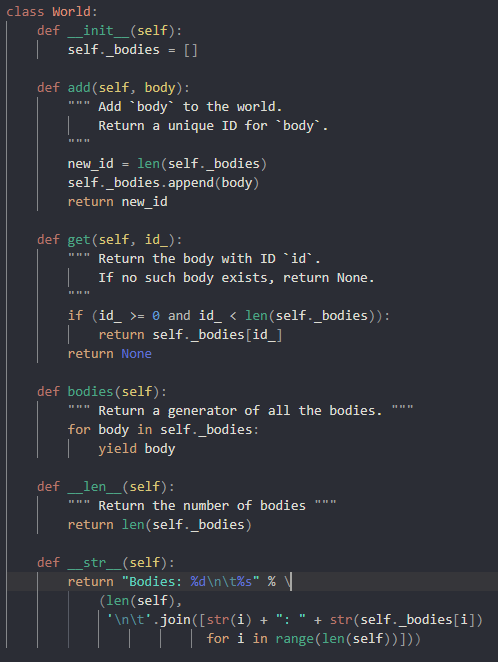
\includegraphics[height=.8\textheight]{World.png}
        \end{column}
        \begin{column}{.5\textwidth}
            This class is used to represent the state of the world, it stores all the bodies in a list and exposes methods to add and get them.
            
            \vspace{1em}
            
            The method \mintinline{python}{bodies} is a \textbf{generator}, it makes it possible to iterate through the list of bodies without actually generating a list in memory. 

            \vspace{1em}
            
            Generators are a useful tool, read the doc: \url{https://wiki.python.org/moin/Generators}
        \end{column}
    \end{columns}
\end{frame}

\begin{frame}{Data structures}{Vector, Vector2}
    \small

    {\centering vector.py \par}

    \vspace{1em}

    \textbf{Vector} represents a vector of dimension n. It overrides the arithmetic operators +, *, - and /, and it defined the \emph{array access} operator \mintinline{python}{[]}.\\
    
    It is used by the solver to represent its state (4 dimension per body: $x$,$y$,$v_x$ and $v_y$).\\

    \textbf{Vector2} inherits from Vector and is a version that represents vectors of dim. 2. In particular it can be initialized using its constructor: \mintinline{python}{Vector2(x, y)}, it also provides getters and setters methods for $x$ and $y$: \mintinline{python}{get_x}, \mintinline{python}{get_y}, \mintinline{python}{set_x} and \mintinline{python}{set_y}.\\

    It is used by \mintinline{python}{Body} to represent its position and velocity, by \mintinline{python}{Screen} to represent its size and by \mintinline{python}{Camera} to represent its position.
\end{frame}

\begin{frame}\centering\huge Problem 2: Modularity\end{frame}

\begin{frame}[fragile]{Problem 2: Modularity}
    
    A well thought program is composed of different modules with well-defined interfaces.\\

    Modules should not care about the implementation of other modules.\\

    This way, any functionality can be reimplemented without affecting other ones.
    
\end{frame}

\begin{frame}[fragile, allowframebreaks]{Example: Solver}

    In the simple example, I used explicit euler to approximate the dynamics.

    \[\forall n \geq 0, y_{n+1} = y_n + dt * f(t, y_n) \quad \quad y_0 \in \mathbb{R}\]

    Implementation:  
    \begin{minted}{python}
for i in range(len(bodiesX)):
    bodiesX[i] += dt * bodiesVX[i]
    bodiesY[i] += dt * bodiesVY[i]
    bodiesVX[i] += dt * bodiesAX[i]
    bodiesVY[i] += dt * bodiesAY[i]
    \end{minted}

    \framebreak
    
    \textbf{Leapfrog integration}:\\
    with $x_i$ the positions, $v_i$ the velocities and $a_i$ the accelerations: 
    \[\forall n \geq 0, 
    \begin{array}{l}
        v_{i+1} = v_i + \frac{h}{2} (a_i + a_{i+1}) \\
        x_{i+1} = x_i + h * v_i + \frac{h^2}{2} * a_i \\
    \end{array}\]

    This method needs $a_i$ and $a_{i+1}$ to compute the state of the system at step $i+1$. We would need to update the code to keep track of the last accelerations that we computed.\\

    But how could we implement both methods, and switch between them easily ? This is what modularity is about.\\
    \textbf{We should use classes !}

\end{frame}

\begin{frame}{Modularity: Interfaces}
    
    Historically called facade pattern, it is a very powerful \textbf{pattern design}, (cf Beck, Kent; Cunningham, Ward (September 1987). \textit{Using Pattern Languages for Object-Oriented Program}. OOPSLA '87 workshop).\\
    
    An interfaces is a description of the methods that a class \textbf{must} implement. A modular code should have well-defined interfaces.\\
    Additionally, interfaces allows to decouple the code: a module A that needs the features of a module B should depend on the \emph{interface} of B, not an implementation.\\
    
    In some languages, there is a primitive way to implement interfaces, \textbf{but not in python}.
\end{frame}
    
\begin{frame}[fragile]{Modularity: Interfaces}{Example}
    
    In the skeleton code for this project, interfaces are classes with a name that starts with I, their methods are not implemented. \\
    {\small Example:
    \begin{minted}{python}
class IEngine:
    def __init__(self, world):
        self.world = world

    def derivatives(self, t0, y0):
        raise NotImplementedError

    def make_solver_state(self):
        raise NotImplementedError
    \end{minted}
    }

    \textbf{DO NOT} modify the code of this interface, if you want to implement an engine, you should create a new class and inherit from \mintinline{python}{IEngine} and reimplement the methods \mintinline{python}{derivatives} and \mintinline{python}{make_solver_interface}

\end{frame}

\begin{frame}\centering\huge A modular approach to the problem\end{frame}

\begin{frame}{A modular approach to the problem}{Solver}
    {
        \centering
        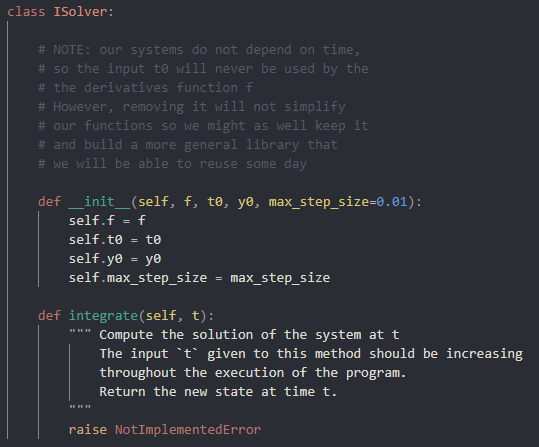
\includegraphics[height=.6\textheight]{ISolver.png}
        \par
    }

    This is the ODE solver, the \mintinline{python}{integrate} method computes the dynamic of the system until time \mintinline{python}{t}.

\end{frame}

\begin{frame}[allowframebreaks]{A modular approach to the problem}{Engine}
    {
        \centering
        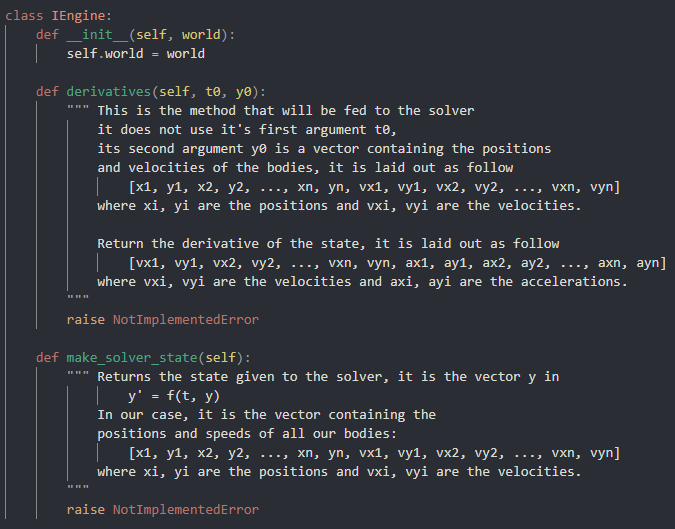
\includegraphics[height=.8\textheight]{IEngine.png}
        \par
    }

    \framebreak

    This is the physics engine, given the positions and velocities of the planets (\mintinline{python}{y0}) and their characteristics (stored in \mintinline{python}{world}), it computes their accelerations.\\

    \mintinline{python}{make_solver_state} is used to convert from the representation used by the engine (\mintinline{python}{world} of type \mintinline{python}{World}) to the representation used by the solver (a \mintinline{python}{Vector} with 4 dimension per body).
\end{frame}

\begin{frame}[fragile]{A modular approach to the problem}{Simulator}
    {
        \centering
        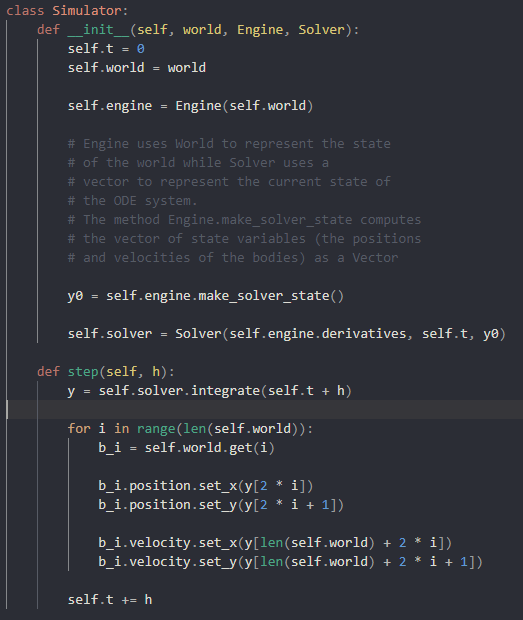
\includegraphics[height=.6\textheight]{Simulator.png}
        \par
    }
    
    This is the main class of the program. It instantiates an engine and a solver and exposes a \mintinline{python}{step} function that simulates \mintinline{python}{h} seconds.
    
    This concludes the logic part, we still need to handle the graphics.
\end{frame}

\begin{frame}[fragile]{A modular approach to the problem}{Camera}
    {
        \centering
        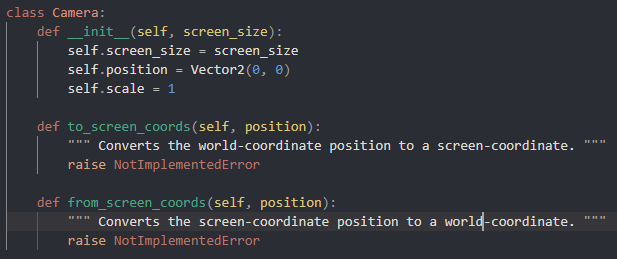
\includegraphics[width=\textwidth]{Camera.png}
        \par
    }
    
    This very simple class handles makes it possible to move and scale the view easily, it implements a base change from the coordinate system of the world to the one defined by \mintinline{python}{self.position} and \mintinline{python}{self.scale}.
\end{frame}

\begin{frame}[fragile]{A modular approach to the problem}{Screen}    
    I implemented a basic screen class to help you get started. You must refer to \href{https://www.pygame.org/docs/}{pygame documentation} to implement new features.\\

    I \textbf{do not} expect you to test this class.
\end{frame}

\begin{frame}\centering\Huge Tests\end{frame}

\begin{frame}{Tests}
    Some tests are already provided, once you implement all the missing methods, you should pass all the tests.\\
    These tests are also a good example of how the features are used, take a look.

    \vspace{1em}

    Additionally, testing is an important part of software development, write your own tests as you write new features.\\
    Remember: tests should be about interfaces, not implementations. You should always check that a feature does \textbf{what} it is supposed to do, not \textbf{how} it does it.\\
    In particular, you should not be testing internal methods of a class as they are implementation details that should be irrelevant.
\end{frame}

\begin{frame}{}{}
    {\centering\Huge Second step \par}

    \vspace{1em}

    Implement a better solver, a faster physics engine, a better screen, with more features, find stable orbits, etc..\\

    cf sujet.pdf    
\end{frame}

\end{document}